\section{Hybrid Dynamics and Event Detection}
The tractor-winch-sled system presented has certain physical limitations that require multiple dynamic states relating to braking, cable tension, and the minimum and maximum cable length. This motivates the need to detect certain events in each operating mode so that smooth and accurate transitions can occur between different dynamics. Figure \ref{fig:Hybrid_Dynamics_State_Machine} presents a state machine where each state is described by whether or not there is tension in the cable, the winch is locked or unlocked, the governing dynamics, and the position of the four-way two-position valve. The dynamics number matches the subscripts denoted for the equations of motion in each state.
\begin{figure}[htb]
    \centering
    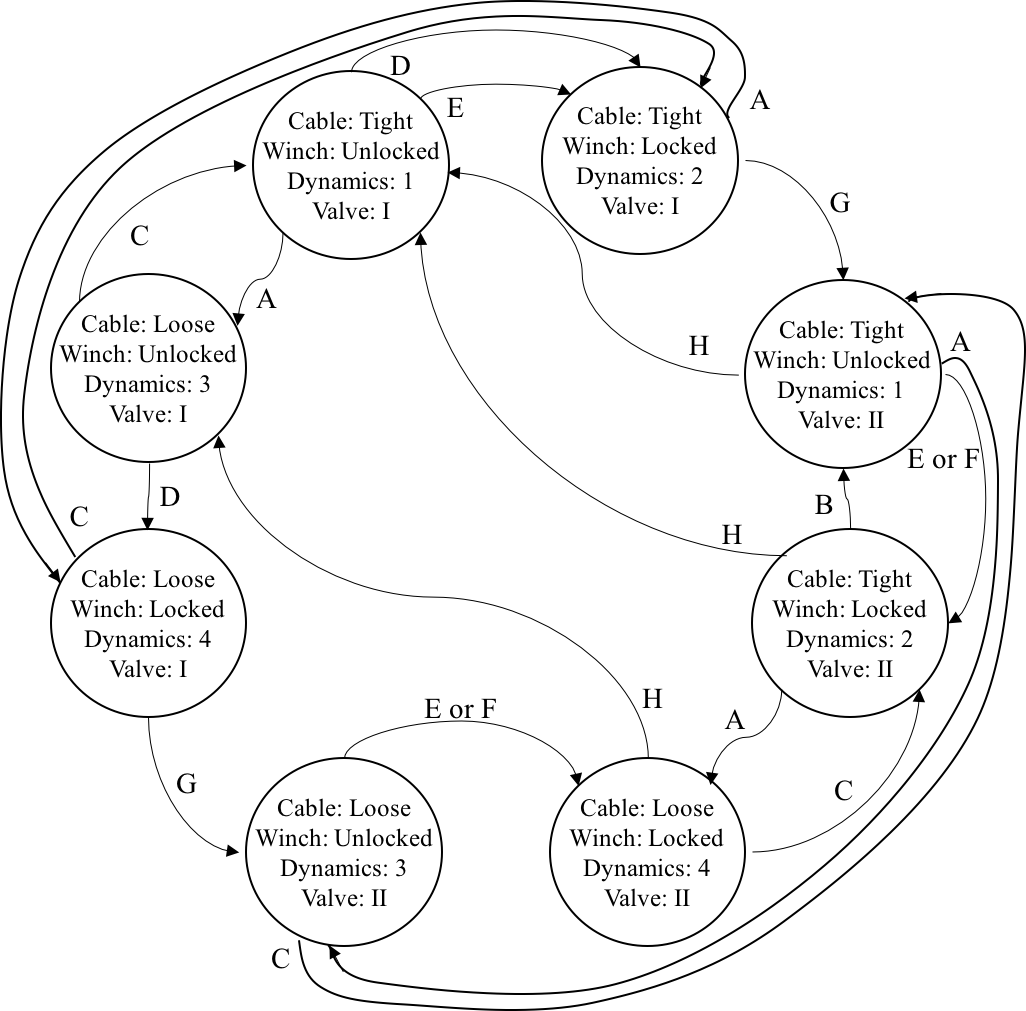
\includegraphics[width = 4in, keepaspectratio]{Hybrid_Dynamics_State_Machine}
    \vspace{-5pt}
    \centering
    \begin{myitemize}
        \footnotesize
        \item A. \hspace{0.1cm} $DB \geq 0 \rightarrow DB \leq 0$
        \item B. \hspace{0.1cm} $\tau_W \geq r_WDB \rightarrow \tau_W < r_WDB $
        \item C. \hspace{0.1cm} $X_{SD} + \psi r_W > X_T \rightarrow X_{SD} + \psi r_W \leq X_T$
        \item D. \hspace{0.1cm} $\psi \geq 0 \rightarrow \psi < 0$
        \item E. \hspace{0.1cm} $\psi r_W < L_C \rightarrow \psi r_W \geq L_C$
        \item F. \hspace{0.1cm} $\dot\psi > 0 \rightarrow \dot\psi \leq 0$
        \item G. \hspace{0.1cm} I $\rightarrow$ II
        \item H. \hspace{0.1cm} II $\rightarrow$ I
    \end{myitemize}
    \vspace{-10pt}
    \caption{State machine for hybrid dynamics of the tractor-winch-sled system. Events triggering transitions are letted A-H below the state machine with their respective criteria.}
    \vspace{-10pt}
    \label{fig:Hybrid_Dynamics_State_Machine}
\end{figure}
The events that trigger state changes are lettered A-H with criteria at the bottom of Fig. \ref{fig:Hybrid_Dynamics_State_Machine}. These criteria are written in a way that directly corresponds to how they are programmed in simulations. In this study, simulations are programmed in MATLAB and use the ODE45 solver with two function callbacks. One callback defines the dynamics of the system while the other defines the events for state changes based on whether or not a zero crossing is detected for a defined expression. There is also an option to specify the direction of the zero crossing. Once an event has been detected integration is terminated, a flag is set for the governing dynamics, and then the simulation proceeds using the correct equations of motion.

